\chapter{Brief Compendium of Neutron Diffusion Benchmarks}
\label{ap:benchmarks}

\section{Introduction}
\section{Two Dimension}
  \subsection{VVER440}
    \begin{figure}
      \centering
      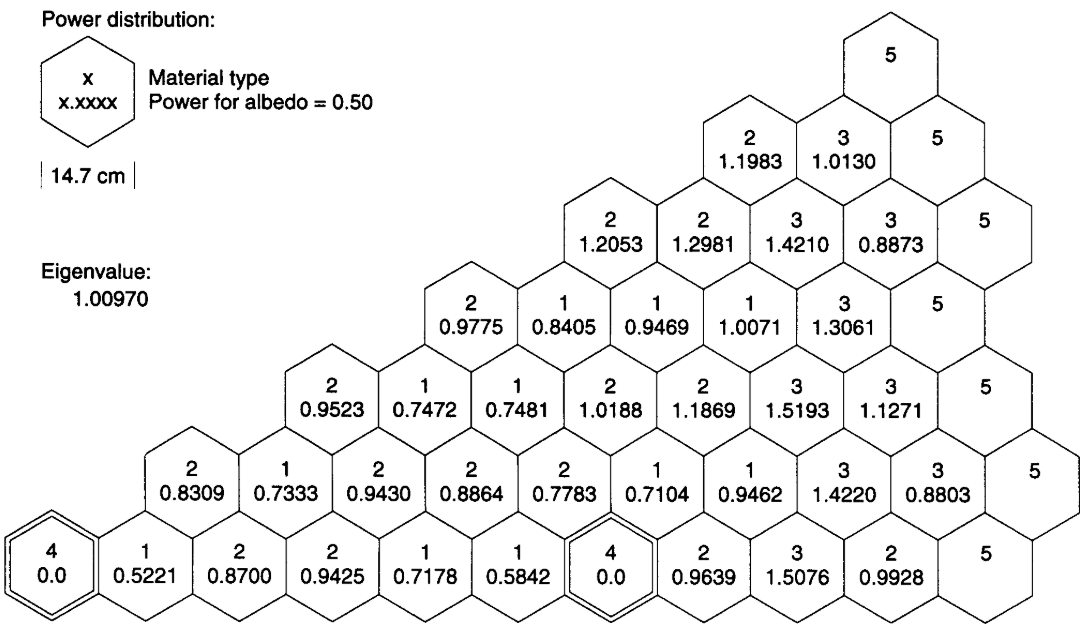
\includegraphics[width=0.6\textwidth]{vver440_geom}
      \caption{VVER440 Geometry \cite{chao}.}
      \label{fig:vver440_geom}
    \end{figure}
    \begin{table}
      \caption{VVER440 Cross Sections.}
      \label{tab:vver440xs}
      \begin{center}
        \begin{tabular}{cccccc}
          \toprule
          &MAT1&MAT2&MAT3&MAT4&MAT5\\
          \midrule
          $D_1$&1.346600E+00&1.337700E+00&1.332200E+00&1.195300E+00&1.448500E+00\\
          $D_2$&3.716900E-01&3.691800E-01&3.650200E-01&1.931300E-01&2.517600E-01\\
          $\Sigma_{r1}$&2.525500E-02&2.470900E-02&2.435000E-02&3.563600E-02&3.318400E-02\\
          $\Sigma_{r2}$&6.427700E-02&7.936100E-02&1.001000E-01&1.349800E-01&3.283900E-02\\
          $\Sigma_{s 1\rightarrow 2}$&1.689300E-02&1.591200E-02&1.488800E-02&2.226400E-02&3.226200E-02\\
          $ \nu \Sigma_{f1}$&4.448800E-03&5.533700E-03&7.039100E-03&&\\
          $ \nu \Sigma_{f2}$&7.375300E-02&1.058100E-01&1.496400E-01&&\\
          \bottomrule
        \end{tabular}
      \end{center}
    \end{table}
  \subsection{SNR}
    \begin{figure}
      \centering
      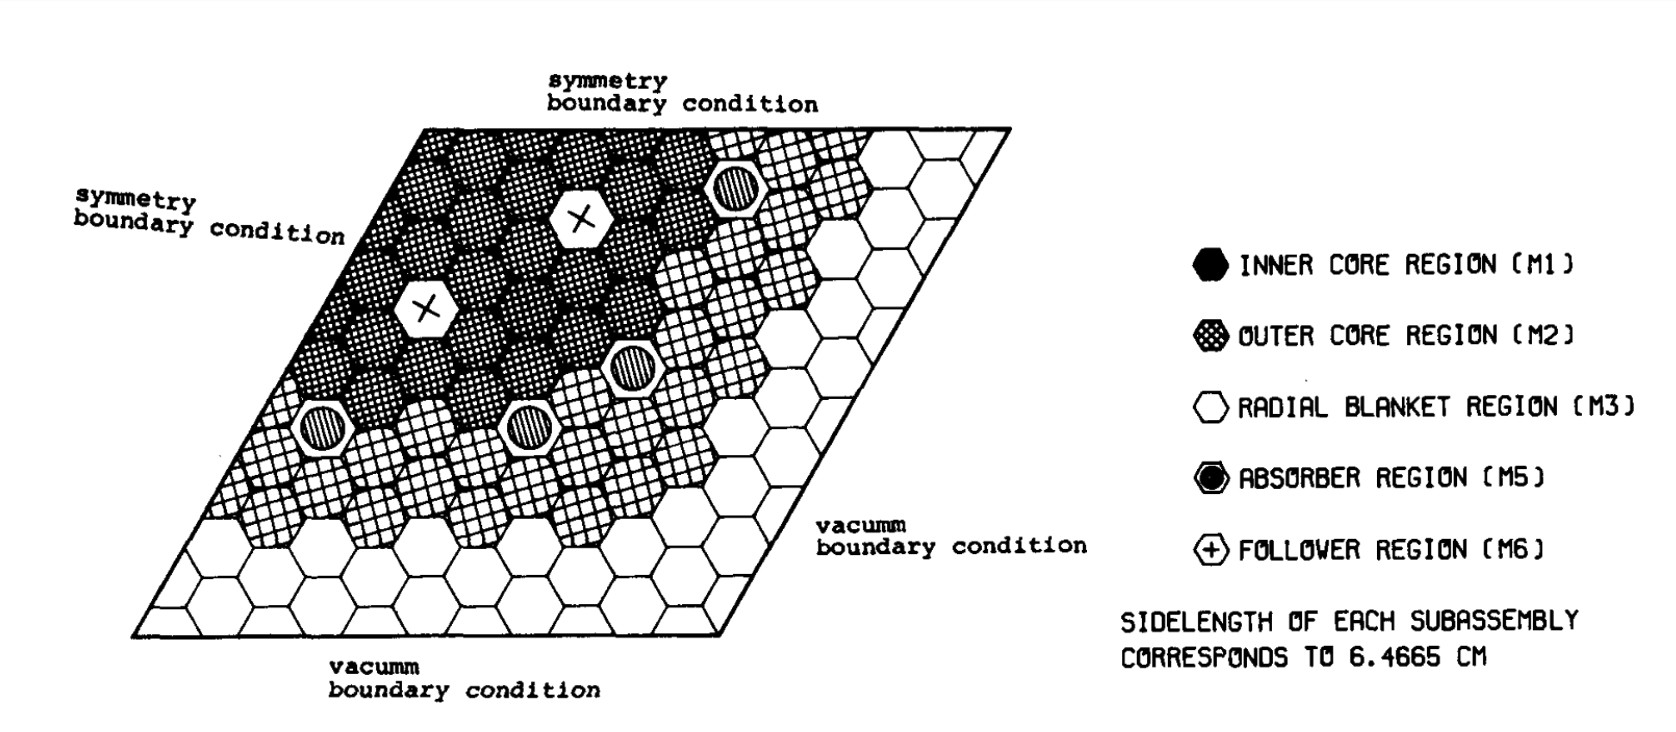
\includegraphics[width=0.6\textwidth]{snr_geom}
      \caption{SNR Geometry \cite{argonneBenchmark}.}
      \label{fig:snr_geom}
    \end{figure}
    \begin{table}
      \caption{SNR Cross Sections.}
      \label{tab:snrxs}
      \begin{center}
        \begin{tabular}{ccccccc}
          \toprule
          &I1&I2&I3&I4&I5&I6\\
          \midrule
          $D_1$&2.876787E+00&2.876539E+00&2.285610E+00&2.716653E+00&2.503066E+00&4.616422E+00\\
          $D_2$&1.570845E+00&1.571363E+00&1.171935E+00&1.440943E+00&1.314665E+00&2.901831E+00\\
          $D_3$&7.224859E-01&7.127076E-01&6.324751E-01&7.203469E-01&5.742770E-01&1.021179E+00\\
          $D_4$&9.641993E-01&9.429781E-01&8.183574E-01&9.876836E-01&6.153695E-01&1.729625E+00\\
          $\Sigma_{r1}$&2.820400E-02&2.878200E-02&3.595900E-02&2.909300E-02&2.481400E-02&1.315900E-02\\
          $\Sigma_{r2}$&5.274700E-03&6.049100E-03&5.885500E-03&4.490900E-03&1.641200E-02&1.455900E-03\\
          $\Sigma_{r3}$&1.761200E-02&1.951000E-02&1.604100E-02&1.308200E-02&7.212200E-02&4.600100E-03\\
          $\Sigma_{r4}$&2.654600E-02&3.371400E-02&1.334900E-02&9.956200E-03&1.686800E-01&7.866000E-04\\
          $\Sigma_{s 1\rightarrow 2}$&2.359700E-02&2.326200E-02&3.207100E-02&2.632200E-02&2.294600E-02&1.294200E-02\\
          $\Sigma_{s 1\rightarrow 3}$&4.079100E-06&4.645100E-06&3.888000E-06&2.890700E-06&1.032000E-06&6.878000E-07\\
          $\Sigma_{s 2\rightarrow 3}$&1.615300E-03&1.571800E-03&2.777600E-03&2.288900E-03&3.768700E-03&1.287100E-03\\
          $\Sigma_{s 1\rightarrow 4}$&4.449300E-08&4.996800E-08&4.503900E-08&3.324800E-08&1.048900E-08&6.990300E-09\\
          $\Sigma_{s 2\rightarrow 4}$&4.230900E-08&4.072400E-08&9.001800E-08&6.213300E-08&7.036100E-12&4.363300E-12\\
          $\Sigma_{s 3\rightarrow 4}$&4.683800E-03&4.341400E-03&5.897100E-03&5.353600E-03&8.681500E-03&3.453300E-03\\
          $ \nu \Sigma_{f1}$&1.187800E-02&1.494300E-02&7.742700E-03&5.427900E-03&&\\
          $ \nu \Sigma_{f2}$&5.325200E-03&7.688700E-03&1.082500E-04&7.585700E-05&&\\
          $ \nu \Sigma_{f3}$&1.047100E-02&1.480900E-02&2.974200E-04&2.121799E-04&&\\
          $ \nu \Sigma_{f4}$&2.661100E-02&3.815900E-02&8.468699E-04&5.759200E-04&&\\
          \bottomrule
        \end{tabular}
      \end{center}
    \end{table}
  \subsection{IAEA}
    \begin{figure}
      \centering
      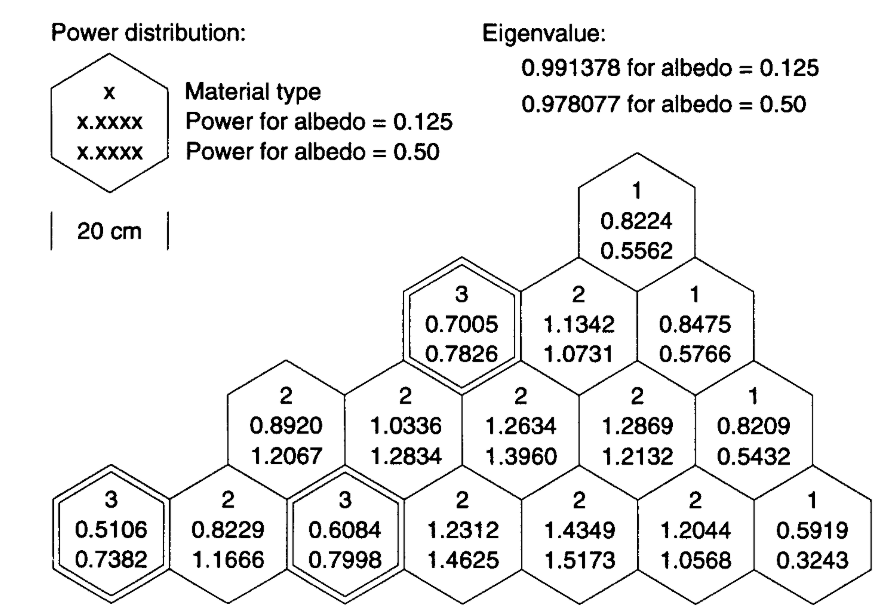
\includegraphics[width=0.6\textwidth]{iaea_nore_geom}
      \caption{IAEA Without Reflector Geometry \cite{chao}.}
      \label{fig:iaea_nore_geom}
    \end{figure}
    \begin{figure}
      \centering
      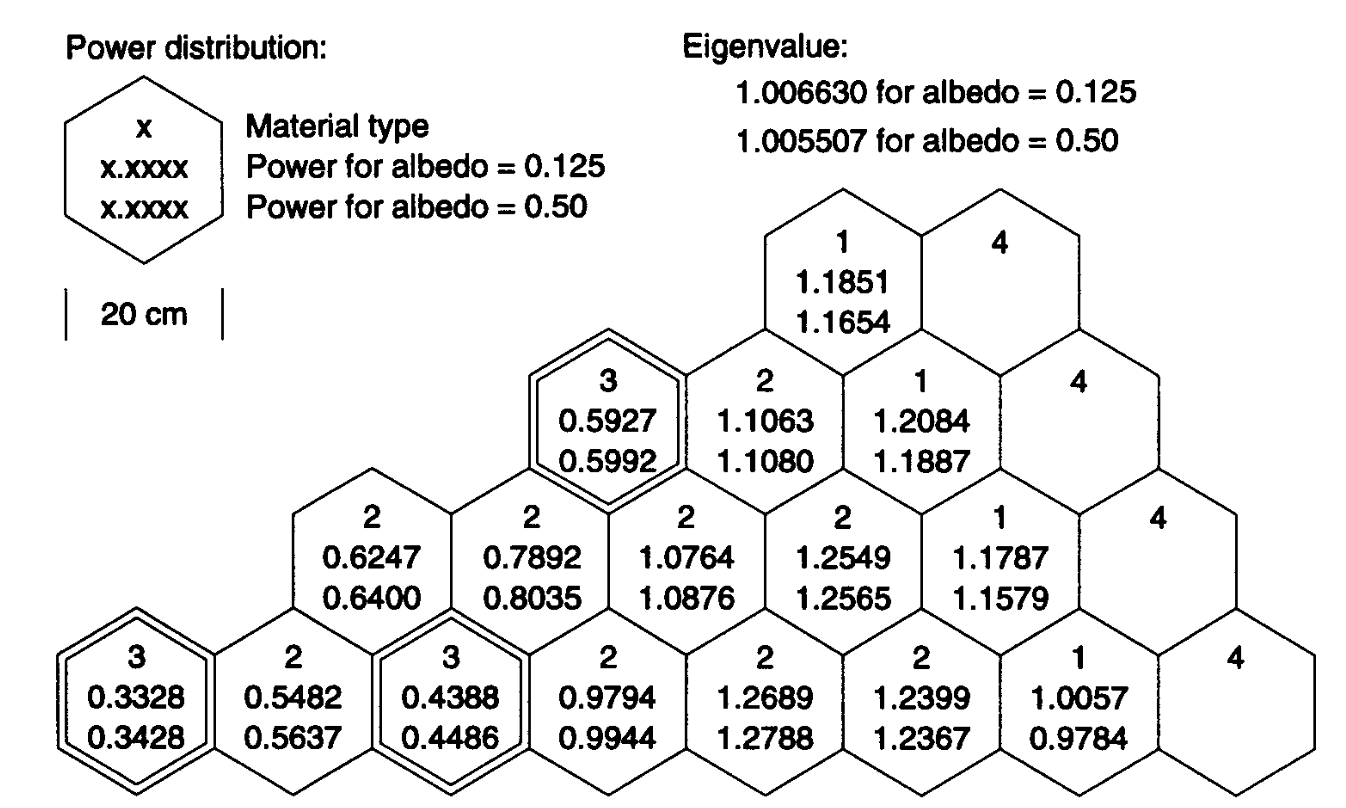
\includegraphics[width=0.6\textwidth]{iaea_refl_geom}
      \caption{IAEA With Reflector Geometry \cite{chao}.}
      \label{fig:iaea_refl_geom}
    \end{figure}
    \begin{table}
      \caption{IAEA Cross Sections.}
      \label{tab:iaeaxs}
      \begin{center}
        \begin{tabular}{ccccc}
          \toprule
          &MAT1&MAT2&MAT3&REFL\\
          \midrule
          $D_1$&1.500001E+00&1.500000E+00&1.500001E+00&1.500000E+00\\
          $D_2$&4.000001E-01&4.000000E-01&4.000001E-01&4.000000E-01\\
          $\Sigma_{r1}$&3.000000E-02&3.000000E-02&3.000000E-02&4.000000E-02\\
          $\Sigma_{r2}$&8.000000E-02&8.500000E-02&1.300000E-01&1.000000E-02\\
          $\Sigma_{s 1\rightarrow 2}$&2.000000E-02&2.000000E-02&2.000000E-02&4.000000E-02\\
          $ \nu \Sigma_{f1}$&&&&\\
          $ \nu \Sigma_{f2}$&1.350000E-01&1.350000E-01&1.350000E-01&\\
          \bottomrule
        \end{tabular}
      \end{center}
    \end{table}
\section{Three Dimension}
  \subsection{MONJU}
    \begin{table}
      \caption{MONJU Cross Sections.}
      \label{tab:monjuxs}
      \begin{center}
        \begin{tabular}{cccccc}
          \toprule
          &IC&OC&RB&CR&NA\\
          \midrule
          $D_1$&2.540000E+00&2.547990E+00&2.173000E+00&2.500010E+00&4.805000E+00\\
          $D_2$&1.724000E+00&1.725000E+00&1.439000E+00&1.681000E+00&3.262000E+00\\
          $D_3$&1.264000E+00&1.269000E+00&1.026000E+00&1.269000E+00&2.431000E+00\\
          $\Sigma_{r1}$&3.098650E-02&3.121380E-02&3.793080E-02&2.328030E-02&1.152508E-02\\
          $\Sigma_{r2}$&9.490000E-03&9.875000E-03&1.184300E-02&1.272700E-02&3.648740E-03\\
          $\Sigma_{r3}$&7.333000E-03&8.099000E-03&7.611000E-03&1.497000E-02&3.072000E-04\\
          $\Sigma_{s 1\rightarrow 2}$&2.544000E-02&2.497000E-02&3.288000E-02&2.185000E-02&1.130000E-02\\
          $\Sigma_{s 1\rightarrow 3}$&5.625000E-04&5.548000E-04&7.468000E-04&2.163000E-04&6.718000E-05\\
          $\Sigma_{s 2\rightarrow 3}$&6.551000E-03&6.341000E-03&1.000000E-02&9.379000E-03&3.571000E-03\\
          $ \nu \Sigma_{f1}$&1.235000E-02&1.467000E-02&8.631000E-03&&
          $ \nu \Sigma_{f2}$&5.225000E-03&6.955000E-03&5.995000E-04&&
          $ \nu \Sigma_{f3}$&7.684000E-03&9.986000E-03&1.381000E-03&&
          \bottomrule
        \end{tabular}
      \end{center}
    \end{table}
  \subsection{KNK}
    \begin{table}
      \caption{KNK Cross Sections.}
      \label{tab:knkxs}
      \begin{center}
        \begin{tabular}{ccccccccccccc}
          \toprule
          &STEEL&AXBL&AXRF&TEST&DRIV&DRMOD&REFL&RFMOD&KNKREF&NASTL&CRD&NACRD\\
          \midrule
          $D_1$&3.388781E+00&2.373121E+00&2.507529E+00&2.676817E+00&2.377115E+00&2.356912E+00&2.091884E+00&2.395256E+00&2.198131E+00&3.453884E+00&2.396616E+00&4.581354E+00\\
          $D_2$&2.466578E+00&1.477974E+00&1.867089E+00&1.658169E+00&1.460419E+00&1.358360E+00&1.540678E+00&1.349566E+00&2.341120E+00&3.376912E+00&1.461014E+00&3.326083E+00\\
          $D_3$&1.483136E+00&1.019165E+00&1.177228E+00&1.163065E+00&1.023104E+00&8.369847E-01&9.559535E-01&7.367704E-01&2.018587E+00&2.483855E+00&1.045568E+00&2.074220E+00\\
          $D_4$&1.177370E+00&9.768754E-01&7.212400E-01&9.039009E-01&7.968248E-01&7.645435E-01&5.339750E-01&6.215936E-01&4.141579E-01&8.077479E-01&5.313220E-01&2.199117E+00\\
          $\Sigma_{r1}$&7.758804E-03&1.665700E-02&9.938010E-03&1.856200E-02&2.033901E-02&2.709099E-02&1.137701E-02&3.325300E-02&1.321701E-02&8.154706E-03&2.136299E-02&6.395295E-03\\
          $\Sigma_{r2}$&4.558990E-03&8.274010E-03&5.436010E-03&1.165498E-02&1.303201E-02&3.338801E-02&5.945000E-03&6.217301E-02&4.880000E-03&3.460198E-03&3.345301E-02&4.094401E-03\\
          $\Sigma_{r3}$&5.202000E-03&9.116980E-03&5.957010E-03&1.639202E-02&1.892099E-02&4.616198E-02&6.607000E-03&7.935300E-02&4.410000E-03&3.444000E-03&7.445399E-02&4.686990E-03\\
          $\Sigma_{r4}$&2.410000E-03&9.943000E-03&3.569000E-03&4.981199E-02&5.742100E-02&6.511802E-02&4.942950E-03&2.415300E-02&5.912960E-03&3.037990E-03&3.125500E-01&1.207990E-03\\
          $\Sigma_{s 1\rightarrow 1}$&9.060500E-02&1.238050E-01&1.229950E-01&1.059640E-01&1.198870E-01&1.143370E-01&1.479690E-01&1.059110E-01&1.384270E-01&8.835500E-02&1.177220E-01&6.636340E-02\\
          $\Sigma_{s 1\rightarrow 2}$&7.423770E-03&1.454830E-02&9.412310E-03&1.127380E-02&1.307900E-02&2.096640E-02&1.066070E-02&2.964850E-02&1.239010E-02&7.734090E-03&1.260660E-02&6.233930E-03\\
          $\Sigma_{s 2\rightarrow 2}$&1.305810E-01&2.172600E-01&1.730950E-01&1.893700E-01&2.152130E-01&2.120060E-01&2.104100E-01&1.848200E-01&1.375020E-01&9.524930E-02&1.946990E-01&9.612360E-02\\
          $\Sigma_{s 1\rightarrow 3}$&1.181630E-04&1.702760E-04&1.937910E-04&1.461920E-04&1.599380E-04&1.391320E-03&2.499560E-04&3.065020E-03&3.669300E-04&1.947190E-04&1.333140E-04&7.021210E-05\\
          $\Sigma_{s 2\rightarrow 3}$&4.352500E-03&6.788850E-03&5.098810E-03&3.648470E-03&4.001170E-03&2.672690E-02&5.467110E-03&5.917800E-02&4.419270E-03&3.225680E-03&4.322190E-03&4.013750E-03\\
          $\Sigma_{s 3\rightarrow 3}$&2.195470E-01&3.179480E-01&2.771940E-01&2.702070E-01&3.068850E-01&3.520930E-01&3.420850E-01&3.730720E-01&1.607220E-01&1.307560E-01&2.443520E-01&1.560160E-01\\
          $\Sigma_{s 1\rightarrow 4}$&8.258900E-07&9.370830E-07&1.393070E-06&9.621780E-07&1.071660E-06&6.102810E-05&1.825650E-06&1.416970E-04&1.690360E-06&8.896150E-07&1.088390E-06&4.163880E-07\\
          $\Sigma_{s 2\rightarrow 4}$&3.416750E-07&6.047930E-06&7.050750E-07&1.068880E-06&1.827160E-06&1.081860E-03&1.001570E-06&2.692290E-03&1.632800E-06&7.984940E-07&1.854910E-07&1.269390E-07\\
          $\Sigma_{s 3\rightarrow 4}$&4.645940E-03&4.387820E-03&5.096010E-03&1.804790E-03&1.673410E-03&3.290300E-02&5.368790E-03&7.813260E-02&3.330750E-03&2.904810E-03&3.687810E-04&4.491110E-03\\
          $\Sigma_{s 4\rightarrow 4}$&2.807070E-01&3.312810E-01&4.585980E-01&3.189600E-01&3.609060E-01&3.708720E-01&6.193060E-01&5.121030E-01&7.989320E-01&4.096320E-01&3.148160E-01&1.503680E-01\\
          $ \nu \Sigma_{f1}$&&2.961000E-03&&1.790430E-02&1.598780E-02&1.016630E-02&&&&&&
          $ \nu \Sigma_{f2}$&&6.561700E-05&&1.599610E-02&1.644460E-02&9.463600E-03&&&&&&
          $ \nu \Sigma_{f3}$&&1.146300E-04&&2.408560E-02&2.714500E-02&1.873250E-02&&&&&&
          $ \nu \Sigma_{f4}$&&4.934825E-04&&7.331050E-02&8.458075E-02&8.253350E-02&&&&&&
          \bottomrule
        \end{tabular}
      \end{center}
    \end{table}

